% LATEX TEMPLATE 
% adapted from https://infinitedescent.xyz/latex/ by wade_

\documentclass[11pt]{article}

% Edit the following to change the title, author name and date
\title{Calc in 3d Notes}
\author{saffron\_}
\date{}

% Packages
\usepackage{amsmath}
\usepackage{amsfonts}
\usepackage{amssymb}
\usepackage{amsthm}
\usepackage{enumerate}
\usepackage{geometry}
\usepackage{graphicx}
\usepackage{hyperref}
\usepackage{multicol}
% \usepackage[colorlinks=true,linkcolor=magenta]{hyperref}

% Page setup
\setlength{\parskip}{10pt}
\setlength{\parindent}{0pt}
\geometry{
    paper={letterpaper}, % Change to 'a4paper' for A4 size
    marginratio={1:1},
    margin={1in}
}

% Theorem environments
\theoremstyle{definition}
\newtheorem{theorem}{Theorem}
\newtheorem{lemma}[theorem]{Lemma}
\newtheorem{corollary}[theorem]{Corollary}
\newtheorem{proposition}[theorem]{Proposition}
\newtheorem{definition}[theorem]{Definition}
\newtheorem{example}[theorem]{Example}

% Custom per each document
\newcommand{\addsection}[1]{\section*{#1}\addcontentsline{toc}{section}{#1}} % for adding \section*{} sections to \tableofcontents
\newcommand{\bb}[1]{\mathbb{#1}} % love of my life
% \newcommand{\floor}[1]{\left\lfloor #1 \right\rfloor}
% \newcommand{\ceil}[1]{\left\lceil #1 \right\rceil}
\newcommand{\col}[1]{\begin{minipage}{\columnwidth}#1\end{minipage}}
\newcommand{\magn}[1]{\left\lVert #1 \right\rVert}
\DeclareMathOperator{\proj}{proj}
\DeclareMathOperator{\comp}{comp}

\graphicspath{ {./media/} }

\begin{document}
\maketitle
\tableofcontents

%%%%%%%%%%%%%%%%%%%%%%%%%%%%
%% Start of document body %%
%%%%%%%%%%%%%%%%%%%%%%%%%%%%

\newpage
\addsection{Chapter 2: Vectors in Space}

\begin{multicols}{2}[Graphing]
  \col{
    \centering
    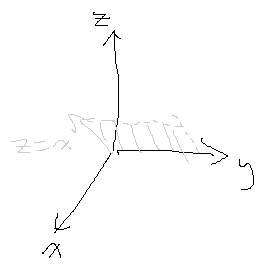
\includegraphics{3d_space.png}
    \emph{convention}
  }
  \col{
    \centering
    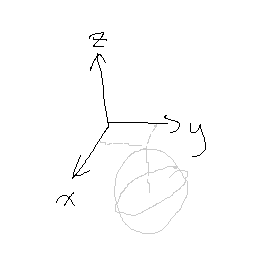
\includegraphics{sphere.png}
    \emph{sphere:} $(x-1)^2 + (y-2)^2 + (z+3)^2 = 9$
  }
\end{multicols}

\begin{multicols}{2}[The Vector]
  \col{
    \centering
    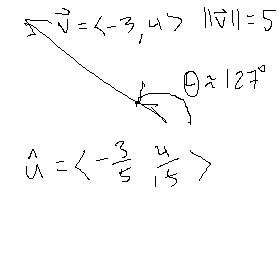
\includegraphics{vector.png}
  }
  \col{
    \begin{itemize}
      \item a quantity with a magnitude and direction
      \item unit vector $\displaystyle\hat{u} =\frac{\vec{v}}{\lVert \vec{v} \rVert}$
    \end{itemize}
  }
\end{multicols}

\newpage
\begin{multicols}{3}[Vector Operations]
  \col{
    \begin{itemize}
      \item Addition
      \begin{itemize}
        \item $\vec{a} = \left< 1,2 \right>$,  $\vec{b} = \left< 3,4 \right>$
        \item $\vec{a} + \vec{b} = \left< 4,6 \right>$
      \end{itemize}
    \end{itemize}
  }
  \col{
    \begin{itemize}
      \item Scalar Multiplication
      \begin{itemize}
        \item $\vec{v} = \left< 1,3 \right>$, $c = 2$
        \item $c\vec{v} = \left< 2,6 \right>$
      \end{itemize}
    \end{itemize}
  }
  \col{
    simple inverses for subtraction and scalar division exist.
  }
\end{multicols}
\begin{multicols}{2}
  \col{
    \begin{itemize}
      \item Dot Product (also 2d!)
      \begin{itemize}
        \item geom.:
        
        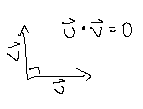
\includegraphics{dot_prod.png} \\
        $\vec{u} \cdot \vec{v} = \magn{\vec{u}} \magn{\vec{v}}\cos \theta$
        \item alg.:
        
        $\vec{u} = \left< u_1, u_2, u_3 \right>$, 
        $\vec{v} = \left< v_1, v_2, v_3 \right>$\\
        $\vec{u} \cdot \vec{v} = \sum u_i v_i$
        \item $\vec{v}\cdot\vec{v} = \magn{\vec{v}}^2$
        \item two vectors are orthogonal aka $\perp$ iff their dot product is $0$
        \item $\displaystyle\cos \theta = \frac{\vec{u} \cdot \vec{v}}{\magn{u}\magn{v}}$ wtf is equation 2.5 "unique over this range" on abt
        \item work $= \vec{F} \cdot \vec{D}$
        \item $\comp$ (scalar projection)
        \begin{align*}
          \comp_{\vec{u}} \vec{v} & = \magn{\vec{v}} \cos \theta \\
          & = \frac{\vec{u} \cdot \vec{v}}{\magn{\vec{u}}}
        \end{align*}
        \item $\proj$ (vector projection)
        \begin{align*}
          \proj_{\vec{u}} \vec{v} &= \comp_{\vec{u}} \vec{v} \cdot \frac{\vec{u}}{\magn{\vec{u}}} \\
          &= \frac{\vec{u}\cdot\vec{v}}{\magn{\vec{u}}^2}\vec{u}
        \end{align*}
      \end{itemize}
    \end{itemize}
  }
  \col{
    \begin{itemize}
      \item Cross Product (3d)
      \begin{itemize}
        \item geom.:
        
        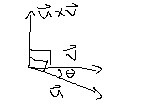
\includegraphics{cross_prod.png}\\
        $\magn{\vec{u}\times\vec{v}} = \magn{\vec{{u}}}\magn{\vec{v}}\sin\theta$
        \item alg.:
        \item $\vec{u} \times \vec{v} = \det\begin{vmatrix}
          \hat{\imath} & \hat{\jmath} & \hat{k}\\
          u_1 & u_2 & u_3 \\
          v_1 & v_2 & v_3
        \end{vmatrix}$
        \item result is $\perp$ to both input vectors, \\
        direction by right hand rule
        \item triple scalar product: \\
        $\vec{u} \cdot (\vec{v}\times\vec{w}) \\ 
        = (\vec{u}\times\vec{v})\cdot\vec{w} \\
        = \det\begin{vmatrix}
          u_1 & u_2 & u_3 \\
          v_1 & v_2 & v_3 \\
          w_1 & w_2 & w_3
        \end{vmatrix}$
        \item if $\vec{u}$ and $\vec{v}$ are the sides of a parallelogram, then its area is $\magn{\vec{u}\times\vec{v}}$
        \item if a parallelepiped has edges $\vec{u}, \vec{v}, \vec{w}$, its volume is the absolute value of its triple scalar product
        \item torque $= \vec{\tau} = \vec{r} \times \vec{F}$
      \end{itemize}
    \end{itemize}
  }
\end{multicols}

\newpage
\begin{multicols}{2}
  \col{
    Lines
    \begin{enumerate}[(1)]
      \item Vector Equation Form
      
      $\vec{r} = \vec{r_0} + t\vec{v}$ \\
      eg $\left<x,y,z\right> = \left<1,2,-5\right> + t\left<3,-4,-1\right>$
      \item Parametric Equation Form
      \begin{align*}
        x &= 1+3t \\
        y &= 2-4t \\
        z &= -5-t 
      \end{align*}
      
      \item Symmetric Equation Form 
      
      solve for $t$
      \[\frac{x-1}{3} = \frac{y-2}{-4} = \frac{z+5}{-1}\]

      \item Edge Case: 0-component
      
      Let a line be defined by the point and vector $(1,-2,6)$ and $\left<3,7,0\right>$. We say the line is:
      \[ \frac{x-1}{3} = \frac{y+2}{7}, z=6 \]
    \end{enumerate}
    \begin{itemize}
      \item point to line distance: use paralleogram area trick
    \end{itemize}

    Planes
    \begin{enumerate}[(1)]
      \item Vector Equation Form
      
      $(\vec{r}-\vec{r_0})\cdot \vec{n} = 0$ \\
      eg $(\left<x,y,z\right>-\left<1,0,1\right>) \cdot \left<1,2,-3\right> = 0$
      \item Scalar Equation, "General" Form
      
      $ax +by +cz +d = 0$
    \end{enumerate}
    \begin{itemize}
      \item point to plane distance: use $\comp_{\vec{u}}\vec{v}$ trick
      \item angle between planes: same as angle between their normal vectors
    \end{itemize}

    Quadric Surfaces
    \begin{itemize}
      \item cylinder: 3d shape consisting of all parallel lines (eg $y=3x^2$)
      \item see \url{quadric_surfaces.pdf}
    \end{itemize}
  }
  \col{
    \addsection{Chapter 3: Vector-Valued Functions}
    Vector-Valued Function
    $${\vec{r}(t) = \left<f(t), g(t), h(t)\right>}, i < t < j$$

    Unit Circle Parameterization
    
    temp\\

    Limits of VVFs
    \begin{itemize}
      \item pass them into the vec. pretty intuitive
      \item a VVF $\vec{r}(a)$ is cont. at $a$ iff $\displaystyle\lim_{t\rightarrow a}\vec{r}(t) = \vec{r}(a)$ (and both are defined )
    \end{itemize}

    Calc with VVFs
    \begin{itemize}
      \item derivatives are intuitive. use the corresponding dot/cross/scalar in deriving $\vec{u}\cdot\vec{v}$
      \item unit tangent vector is the derivative's unit vector
      \item integrals are intuitive. consider constant vector $C$ instead of scalar constant
    \end{itemize}

    Consult exam 1 cheatsheet for notes on the rest of the chapter
  }
\end{multicols}

\newpage
\addsection{Chapter 4: Differentiation}
\begin{multicols}{2}
  \col{
    Functions of Multiple Variables
    \begin{itemize}
      \item domain: analyze what values are invalid
      \item range: image of domain
      \item level planes/level surfaces/contour maps: setting the function to some constant and drawing out the resulting shape 
    \end{itemize}

    Limits and Continuity
    \begin{itemize}
      \item limit rules are identical to 2d, including
      \item limits must be unique. ie, the $\delta$ disk around a point must only contain one value. (disprove limit by finding different values through different ``paths'' to the limit)
      \item as in 2d, $f(x,y)$ is continuous at $(a,b)$ iff
      \[  \lim_{(x,y)\rightarrow(a,b)}f(x,y) = f(a,b)\]
      with both defined.
      \item sum, product, comp of cont functions: cont
    \end{itemize}

    Partial Derivatives
    \begin{itemize}
      \item slope of line in a direction, at a point
      \item Limit definition:
      \[ \frac{\partial f}{\partial x} = \lim_{h\rightarrow 0}\frac{f(x+h,y)-f(x,y)}{h}\]
      \item four second order partials exist
      \begin{gather*}
        \frac{\partial^2 f}{\partial x^2} = \frac{\partial}{\partial x}\left[\frac{\partial f}{\partial x}\right] = f_{xx} \\
        \frac{\partial^2 f}{\partial x\partial y} = \frac{\partial}{\partial x}\left[\frac{\partial f}{\partial y}\right] = f_{yx} \\
        \frac{\partial^2 f}{\partial y\partial x} = \frac{\partial}{\partial y}\left[\frac{\partial f}{\partial x}\right] = f_{xy} \\
        \frac{\partial^2 f}{\partial y^2} = \frac{\partial}{\partial y}\left[\frac{\partial f}{\partial y}\right] = f_{yy} \\
      \end{gather*}
      \item Clairaut's Thrm: if $f_{xy}$ and $f_{yx}$ are cont near a point, they are equal
    \end{itemize}
  }
  \col{
    Tangent Planes
    \begin{itemize}
      \item if all tangent lines to a point are in the same plane, call that the tangent plane
      \begin{itemize}
        \item (not true if there is a point)
        \item maybe theres a correlation somewhere with differentiability? (p393)
      \end{itemize}
      \item the tangent plane to $z = f(x,y)$ at $(a,b)$ is 
      \[ z = f(a,b) + f_x(a,b)(x-a) + f_y(a,b)(y-b) \]
      \item find an approx at $(a,b)$ via the linear approximation plane $L(x,y) = $ RHS (above)
      \item a function is differentiable at $(a,b)$ iff
      \[ f(x,y) = \text{RHS} + E(x,y) \]
      where the error term $E$ satisfies
      \[ \lim_{(x,y)\rightarrow(a,b)}\frac{E(x,y)}{\sqrt{(x-a)^2+(y-b)^2}} = 0. \]
      alternatively, if $f$, $f_x$, and $f_y$ exist near $(a,b)$ and are cont. at $(a,b)$, then $f$ is differentiable there.
      \item let $z=f(x,y)$ with $(a,b)$ in the domain of $f$, and let $\Delta x$ and $\Delta y$ be chosen such that $(a+\Delta x,b+\Delta y)$ is also in the domain of $f$.
      
      then
      \begin{gather*}
        dx = \Delta x \\
        dy = \Delta y \\
        dz = f_x(a,b)dx + f_y(a,b)dy.
      \end{gather*}
      $dx$ and $dy$ are differentials, $dz$ the ``total differential,'' and we estimate error with it.

      notice the similarity to the tangent plane equation.
    \end{itemize}
  }
\end{multicols}

\begin{multicols}{2}
  \col{
    The Chain Rule
    \begin{itemize}
      \item consider
      \begin{gather*}
        w=f(x,y,z) \\
        x = x(t,u,v) \\
        y = y(t,u,v) \\
        z = z(t,u,v) \\
        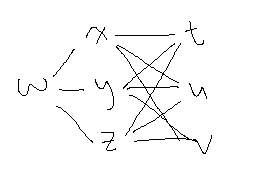
\includegraphics{chain_rule_treediagram.png}.
      \end{gather*}
      then,
      \begin{gather*}
        \frac{\partial w}{\partial t} = 
          \frac{\partial w}{\partial w}\frac{\partial x}{\partial t}
          + \frac{\partial w}{\partial y}\frac{\partial y}{\partial t}
          + \frac{\partial w}{\partial z}\frac{\partial z}{\partial t}.
      \end{gather*}
      others are left as an exercise to the reader.
    \end{itemize}

    Implicit Differentiation
    \begin{itemize}
      \item consider $x^2 + 3y^2 + 4y - 4 = 0$. 
      
      to find $\frac{dy}{dx}$, we may implicitly differentiate this by taking $\frac{d}{dx}$ of both sides and solving.

      but we may also define 
      \[ f(x,y) = x^2 + 3y^2 + 4y - 4, f(x,y) = 0.\]
      with this in mind, suppose $f(x,y)=0$. then,
      \[ \frac{dy}{dx} = -\frac{\partial f/\partial x}{\partial f/\partial y} \]
      and if $f(x,y,z) = 0$,
      \[ \frac{\partial z}{\partial x} = -\frac{\partial f/\partial x}{\partial f/\partial z}, \frac{\partial z}{\partial y} = -\frac{\partial f/\partial y}{\partial f/\partial z}.\]
      these can be derived from the chain rule.
    \end{itemize}
  }
  \col{
    Directional Derivatives and the Gradient
    \begin{itemize}
      \item the directional derivative of $f(x,y)$ in the direction $\hat{u} = \left<\cos\theta, \sin\theta\right>$ is
      \[ D_{\hat{u}}f(a,b) = \lim_{h\rightarrow 0}\frac{f(a+h\cos\theta, b+h\sin\theta)-f(a,b)}{h}\]
      alternatively, if the partials exist,
      \begin{align*}
        D_{\hat{u}}f(x,y) &= f_x(x,y)\cos\theta + f_y(x,y)\sin\theta \\
        &= \left<\,f_x(x,y), f_y(x,y)\,\right> \cdot \hat{u} \\
        % &= [\,f_x(x,y)\hat{\i} + f_y(x,y)\hat{\j}\,] \cdot \hat{u} \\
        &= \nabla f(x,y) \cdot \hat{u}.
      \end{align*}
      \item $\nabla f(x,y)$ is called the gradient and points toward the greatest increase of a function. it's perpendicular to the graph's level curves (if the partials are cont. near the points)
      \item suppose $z=f(x,y)$ diffbl at $(a,b)$.
      \begin{itemize}
        \item if $\nabla f(a,b) = \vec{0}$, then $D_{\hat{u}}f(a,b) = 0$ for any $\hat{u}$
        \item if $\nabla f(a,b) \ne \vec{0}$, then $D_{\hat{u}}f(a,b)$ is max when $\hat{u}$ is in the same direction as $\nabla f(a,b)$.
        
        max of $D_{\hat{u}}f(a,b)$ is $\magn{\nabla f(a,b)}$
        \item if $\nabla f(a,b) \ne \vec{0}$, then $D_{\hat{u}}f(a,b)$ is min when $\hat{u}$ is in the opposite direction as $\nabla f(a,b)$.
        
        min of $D_{\hat{u}}f(a,b)$ is $-\magn{\nabla f(a,b)}$
      \end{itemize}
      \item yes, these work for multivar funcs.
    \end{itemize}    
  }
\end{multicols}

\newpage
\begin{multicols}{2}
  \col{
    Finding Maxima/Minima
    \begin{itemize}
      \item like 2d, critical points $(a,b)$ exist iff
      \begin{itemize}
        \item $f_x(a,b) = f_y(a,b) = 0$ 
        \item or the partials there don't exist
      \end{itemize} 
      \item local extrema are crit points
      \item Second Derivative Test (for 3d calc)
      
      let $z=f(x,y)$ where the first and second order partials are cont near a point $(a,b)$
      \[ D = f_{xx}(a,b)f_{yy}(a,b)-(f_{xy}(a,b))^2 \]
      \begin{itemize}
        \item $D > 0$ and $f_{xx}(a,b) > 0$
        
        $\Rightarrow f$ has a local min at $(a,b)$
        \item $D > 0$ and $f_{xx}(a,b) < 0$
        
        $\Rightarrow f$ has a local max at $(a,b)$
        \item $D < 0$
        
        $\Rightarrow f$ has a saddle point at $(a,b)$
        \item $D = 0$
        
        $\Rightarrow$ the test is inconclusive
      \end{itemize}
      \item to find local extrema:
      \begin{enumerate}
        \item find crit points. discard if a partial DNE
        \item find discriminant $D$ for each point
        \item apply 2nd derivative test
      \end{enumerate}
      \item Extreme Value Theorem

      a cont function on a closed and bounded set has an abs min and abs max in the set
      \item the abs max and abs min will be either at a critical point or on a boundry
      \item to analyze the boundry, consider parameterizing line segments/ellipses or using Lagrange multipliers
    \end{itemize}
  }
  \col{
    Lagrange Multipliers
    \begin{itemize}
      \item Theory: consider an objective function and a constraint function. when they are tangent, their gradients must be in the same direction. so, we say they are different by $\lambda$, the Lagrange multiplier.
      \item Let $f(x,y)$ and $g(x,y)$ have cont partials along $g(x,y)=0$. if $f$ has a local extrema on $g(x,y)=0$ at $(a,b)$ and $\nabla g(a,b) \ne 0$, then
      \[ \nabla f(a,b) = \lambda \nabla g(a,b) \]
      \item to use $\lambda$ (yes, $f$ and $g$ may be fn of 3 vars):
      \begin{enumerate}
        \item find the objective function $f(x,y)$, constraint function $g(x,y)$.
        \item solve for $a$ and $b$ using
        \begin{gather*}
          \nabla f(a,b) = \lambda\nabla g(a,b) \\
          g(a,b)=0
        \end{gather*}
        \item largest value of $f$ will be largest among all $f(a,b)$ found. similar for smallest.
      \end{enumerate}
      \item alternatively, with two constraints:
      
      let obj fn be $w=f(x,y,z)$, and constraint fns $g(x,y,z)=0$, $h(x,y,z)=0$. solve for
      \begin{gather*}
        \nabla f(a,b,c) = \lambda_1\nabla g(a,b,c) + \lambda_2\nabla h(a,b,c) \\
        g(a,b,c) = 0 \\
        h(a,b,c) = 0.
      \end{gather*}
    \end{itemize}
    TODO CLOSED/OPEN SETS AND STUFF
    \begin{itemize}
      \item $S$ is called an open set if every point of S is an interior point.
      \item $S$ is called a closed set if it contains all its boundary points.
    \end{itemize}
  }
\end{multicols}

\newpage
\addsection{Chapter 5: Multiple Integration}
\begin{multicols}{2}
  \col{
    Double Integration
    \begin{itemize}
      \item Consider \\
      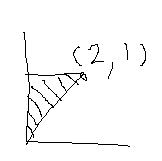
\includegraphics{iint_region.png}.
      \item its area via a double integral:
      \[ \int_{x=0}^{x=2}\int_{y=\frac{1}{2}x}^{2}1dydx.\]
      \item notice the order of bounds variables.
      \item to change order of integration, graph the region to get the bounds ($x$=, $y$=) correct
      \item for improper integrals that come from unbounded functions, adapting the above is fine.
      \item but for improper integrals that come from unbounded regions, consider $\iint xye^{-x^2-y^2}dA$ for the first quadrant. then we set up and solve
      \begin{align*}
        &\,\lim_{(b,d)\rightarrow(\infty, \infty)}\int_{0}^{b}\int_{0}^{d}xye^{-x^2-y^2}dydx \\
        =&\,\lim_{(b,d)\rightarrow(\infty, \infty)}\int_{0}^{b}\int_{0}^{d}xe^{-x^2}ye^{-y^2}dydx \\
        =&\,\lim_{(b,d)\rightarrow(\infty, \infty)}\int_{0}^{b}xe^{-x^2}dx\int_{0}^{b}ye^{-y^2}dy \\
        =&\,\dots \\
        =&\,\frac{1}{4}
      \end{align*}
      \item converting to polar from rectangular? use
      \begin{align*}
        x &=r\cos\theta \\
        y &=r\sin\theta \\
        dA &= rdrd\theta
      \end{align*}
    \end{itemize}
  }
  \col{
    Triple Integration
    \begin{itemize}
      \item six orderings exist for bounds. one ex:
      \begin{gather*}
        \iiint\limits_E f(x,y,z)dV \\
        = \int_{x=a}^{x=b}\int_{y=g_1(x)}^{y=g_2(x)}\int_{z=h_1(x,y)}^{z=h_2(x,y)}f(x,y,z)dzdydx.
      \end{gather*}
      \item think: fix $x$ with first bound. now we can use $x$ in the second bound. etc.
      % \item again, remember to graph surface to better understand changing integration order
      \item avg value of $f$ on region $E$:
      \[ \text{Avg}(f) = \frac{1}{\text{Vol}(E)}\iiint\limits_E f dV \]
      \item rect to cylindrical? just polar, but keep $z$.
      
      $dV = rdzdrd\theta$ is usually best. 
      \item cyl to rect? $r=\sqrt{x^2+y^2}, \tan\theta = y/x$, keep $z$. careful: $\forall \theta,\tan^{-1}(\theta)\in (-\frac{\pi}{2},\frac{\pi}{2})$
      \item consider spherical:\\
      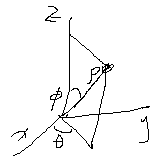
\includegraphics{spherical_coords.png}
      \item rect to spherical: $\rho^2=x^2+y^2+z^2$,\\ $\tan\theta=\frac{y}{x},\phi=\cos^{-1}(\frac{z}{\sqrt{x^2+y^2+z^2}})$
      
      $dV=\rho^2\sin\phi \,d\rho \,d\phi \,d\theta$ usually best
      \item cyl to spherical: $\rho^2 = r^2 + z^2$,\\ $\theta=\theta, \phi=\cos^{-1}(\frac{z}{\sqrt{r^2+z^2}})$
      \item spherical to rect: $x=\rho\sin\phi\cos\theta$, \\$y=\rho\sin\phi\sin\theta,z=\rho\cos\phi$
      \item spherical to cyl: $r=\rho\sin\phi,$\\$\theta=\theta,z=\rho\cos\phi$
    \end{itemize}
  }
\end{multicols}

\begin{multicols}{2}
  \col{
    Centers of Mass, Moments of Inertia
    \begin{itemize}
      \item consider a lamina (2d object). its center of mass $P(\overline{x},\overline{y})$ is defined by
      \[ \overline{x} = \frac{M_y}{m} \text{ and } \overline{y} = \frac{M_x}{m}. \]
      where mass is obtained by integrating $\rho$ over the domain, and moments about the $x$ and $y$ axes are
      \[ M_x = \iint\limits_R y\rho(x,y)dA, M_y = \iint\limits_R x\rho(x,y)dA. \]
      (constant density? $P(\overline{x},\overline{y})$ is the centroid.)
      \item the moments of inertia about the axes are
      \[ I_x = \iint\limits_R y^2\rho(x,y)dA, I_y = \iint\limits_R x^2\rho(x,y)dA \]
      and about the origin (the polar m. of i.):
      \[ I_0 = I_x + I_y = \iint\limits_R (x^2+y^2)\rho(x,y)dA. \]
      (transforming to polar works for all these)
      \item radius of gyration about axes (anal rot?):
      \[ R_x = \sqrt{\frac{I_x}{m}}, R_y = \sqrt{\frac{I_y}{m}}, R_0 = \sqrt{\frac{I_0}{m}} \]
      \item also consider 3d:
      
      for center mass, $\overline{x}=\frac{M_x}{m}, \dots$

      mass $m$ is similar.

      moments about the \emph{axes}:
      \[ M_x=\iiint\limits_Q x\rho(x,y,z)dV, \dots \]
      moments of inertia about the \emph{axes}
      \[ I_x = \iiint\limits_Q (y^2+z^2)\rho(x,y,z)dV, \dots \]
    \end{itemize}
  }
  \col{
    Multivar Change of Variables (like ``$u$-sub'')

    \begin{itemize}
      \item planar transformations
      \begin{itemize}
        \item let $G,R\subseteq \mathbb{R}^2$. a pl. trans. is a fn $T:G\rightarrow R$, transes $G$ region to $R$, via $x=g(u,v), y=h(u,v)$.
        
        (typically assume/require first partials $\exists$ and are cont. ie, $C^1$ trans.)
        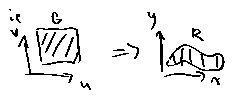
\includegraphics[width=2.7in]{planar_transformations_for_usub.png}
        a trans, $T: G\rightarrow R, T(u,v)=(x,y)$ is one to one iff 2 distinct points cannot map to the same output. ie, $(\forall G_1, G_2\in G)(T(G_1) = T(G_2) \Rightarrow G_1 = G_2)$ 

        if $T$ is one to one, $(\exists T^{-1})(T^{-1}\circ T, T\circ T^{-1})$ are id. fns.

        finding $\text{Im}_T G$? can try eval. each section of $G$'s boundry thru T.
      \end{itemize}
      \item Jacobians:
      \[ J(u,v) = \frac{\partial(x,y)}{\partial(u,v)} = \begin{vmatrix}
        \frac{\partial{x}}{\partial{u}}& \frac{\partial{x}}{\partial{v}} \\
        \frac{\partial{y}}{\partial{u}}& \frac{\partial{y}}{\partial{v}}
      \end{vmatrix}. \]
      The same pattern holds for 3d.
      \item changing variables strategy:
      \begin{enumerate}
        \item sketch integration region ($xy$ plane)
        \item examine region/bounds and integrand, choose $u=\dots, v=\dots$
        \item find bounds in $uv$ plane
        \item evaluate jacobian
        \item substitute bounds, replace $dA$ with $J(u,v)\,du\,dv$.
      \end{enumerate}
    \end{itemize}



  }
\end{multicols}

\newpage
\addsection{Chapter 6: Vector Calc (Exhaustive)}
\begin{multicols}{2}
  \col{
    Conservative Vector Fields
    \begin{itemize}
      \item defns: simple curve: no crossings. simply connected region: no holes.
      \item a vector field $\vec{F}$ is a gradient/conservative vec field iff $\exists f, \nabla f = \vec{F}$
      \begin{itemize}
        \item $f$ is called a potential function
      \end{itemize}
      \item pot. fn. uniqueness is like antiderivs: $\nabla f = \nabla g = \vec{F} \Rightarrow f = g + C$.
      \item cross partial property (prove not cons.):
      \begin{gather*}
        \vec{F} = \left<P, Q, R\right>\text{ is cons.}\\
        \Rightarrow P_y=Q_x \land Q_z=R_y\land R_x=P_z.
      \end{gather*}
      \item to prove it is: use the converse of above, only if $\vec{F}$ is on a open, simply connected region through which the converse holds
    \end{itemize}
    Finding a Potential Function $f$
    \begin{itemize}
      \item given $\vec{F}(x,y)=\left<P,Q\right>$,
    \end{itemize}
    \vspace{-1em}\begin{align}
      f &= \int P \,\partial x + g(y) \text{ ($g$, ``a constant'')} \\
      f_y &= \frac{\partial}{\partial y}(\int P \,\partial x) + g'(y) \text{ taking derivative} \\
      &= Q \text{ by defn of $\vec{F}$, if it has a pot. fn.} 
    \end{align}
    \begin{itemize}
      \item[] solve for $g$, which finishes $f$, via (2) and (3), usually choosing 0 for the constant after antideriv.
    \end{itemize}

    Scalar Line Integrals
    \begin{itemize}
      \item let $f$ be cont with a domain that includes the smooth curve $C$ with parameterization $\vec{r}(t), a\le t\le b$.
      \[ \int_C f\, ds = \int_a^b f(\vec{r}(t))\magn{\vec{r}\,'(t)} dt. \]
      \item idc about reparameterization
      \item $f=1$ finds arclen
    \end{itemize}
  }
  \col{
    Vector Line Integrals
    \begin{itemize}
      \item recall unit tang. vec $\vec{T}=\frac{\vec{r}\,'(t)}{\magn{\vec{r}\,'(t)}}$. since $ds=\magn{\vec{r}\,'(t)}dt$, we may derive
      \[ \int_C \vec{F}\cdot\vec{T}ds = \int_a^b \vec{F}(\vec{r}(t))\cdot\vec{r}\,'(t)dt. \]
      thus, VLIs are often denoted
      \[\int_C \vec{F}\cdot d\vec{r}.\]
      also consider that $\vec{F}=\langle P,Q,R \rangle$ and $d\vec{r}=\left<dx,dy,dz\right>$. so, yet another form:
      \begin{align*}
        &\int_C Pdx + Qdy + Rdz\\
        =&\int P(\vec{r}(t)) \frac{dx}{dt} + Q(\vec{r}(t)) \frac{dy}{dt} + R(\vec{r}(t)) \frac{dz}{dt} dt
      \end{align*}
      \item vector LIs are reversible
      \[\int_{-C}\vec{F}\cdot d\vec{r} = -\int_C \vec{F}\cdot d\vec{r}\]
      \item if an object moves along $C$ in force field $\vec{F}$, the work req'd to move it is $\int_C \vec{F}\cdot d\vec{r}$.
    \end{itemize}
    Flux
    \begin{itemize}
      \item flux of $\vec{F}$ across $C$ measures at what rate fluid crosses a curve.
      \item let $C$ be $\vec{r}(t)=\left<x(t),y(t)\right>, a\le t\le b$.
      
      let $\vec{n}(t) = \left<y'(t),-x'(t)\right>$ (the normal pointing right as we traverse the curve).

      let unit normal vec $\vec{N}(t) = \frac{\vec{n}(t)}{\magn{\vec{n}(t)}}$.

      flux is
      \[\int_C \vec{F}\cdot\vec{N}ds = \int_a^b \vec{F}(\vec{r}(t))\cdot \vec{n}(t)dt\]
      \item notice the similarity:
      \begin{align*}
        \text{circ/LI } & \int_C\vec{F}\cdot\vec{T} ds = \int_C Pdx + Qdy\\
        \text{flux } & \int_C\vec{F}\cdot\vec{N} ds = \int_C -Qdx + Pdy\\
      \end{align*}
    \end{itemize}
  }
\end{multicols}
\newpage
\begin{multicols}{2}
  \col{
    Circulation
    \begin{itemize}
      \item a vector LI along an oriented closed curve is called the circulation of $\vec{F}$ along $C$:
      \[\oint_C \vec{F}\cdot\vec{T} ds \text{ or } \oint_C \vec{F}\cdot d\vec{r}\]
    \end{itemize}
    Fundamental Thrm of Line Integrals
    \begin{itemize}
      \item similarly to the FTC,
      \[\int_C \nabla f \cdot d\vec{r} = f(\vec{r}(b))-f(\vec{r}(a)).\]
      \item so, to find $\int_C \vec{F}\cdot d\vec{r}$,
      \begin{enumerate}
        \item find potential fn (``antiderivative'')
        \item evaluate.
      \end{enumerate}
      \item it follows that if $\vec{F}$ is conserv. (has pot. fn.) and $C$ is closed, $\oint_C \vec{F}\cdot d\vec{r}= 0.$
      \item we also discover path independence: 
      \begin{itemize}
        \item $\vec{F}$ is conserv. $\Rightarrow \vec{F}$ path indep.
        \item ie, work by grav is same for 3 hikers who take diff paths but start/end similarly.
        \item converse is true if domain of $\vec{F}$ is open and connected.
      \end{itemize}
    \end{itemize}
  }
  \col{
    Green's Theorem
    \begin{itemize}
      \item connects a $\iint_D$ to a $\int_C$ around the boundry of $D$.
      \item[] \emph{Circulation Form}
      \item let an open, simply connected region $D$, with piecewise smooth, closed, simple, c.clockwise boundry $C$, with $\vec{F} = \left<P,Q\right>$. (only works with 2D field)
      \[\oint_C\vec{F}\cdot d\vec{r} = \oint_C Pdx + Qdy = \iint_D(Q_x-P_y)dA\]
      \item circulation eq. can be expressed with $\vec{T}$. so, this is also called the ``tangential form''
      \item notice: if $Q_x-P_y=1$, we may use this form to find area. as such, let $\vec{F}=\left<-\frac{y}{2},\frac{x}{2}\right>$. so,
      \[ \text{Area}(D)=\iint_D1dA = \frac{1}{2}\oint_C -ydx+xdy\]
      \item[] \emph{Flux Form}
      \item let an open, simply connected region $D$, with piecewise smooth, closed, simple, c.clockwise boundry $C$, with $\vec{F} = \left<P,Q\right>$.
      \[\oint_C\vec{F}\cdot\vec{N}ds = \oint_C -Qdx+Pdy = \iint_D P_x+Q_y dA.\]
      \item also called the ``normal form''
      \item[] \emph{General Form (holed regions)}
      \item if you have a region with finitely many holes, you may convert the line integral around its boundry into the double integral anyways lmao.
      \item ngl this is so cursed TODO go to OH or tutoring to ask about this. \texttt{https://discord.com/channels/1155614843722805258/1155623088382300282/1228731087644004464} is a link to your thread with ryan about this
    \end{itemize}
  }
\end{multicols}

\newpage
\begin{multicols}{2}
  \col{
    Source-Free Fields
    \begin{itemize}
      \item notice the similarities with conservative fields: $\vec{F}=\left<P,Q\right>$ is a SFF iff \vspace{-0.5em}
      \begin{align*}
        &\text{1. flux} \oint_C\vec{F}\cdot\vec{N}ds = 0\\
        \text{or }&\text{2. flux indep. of path}\\
        \text{or }&\text{3. }\exists\text{ a stream fn } g(x,y) \text{ for } \vec{F}\\
        \text{or }&\text{4. }P_x+Q_y=0
      \end{align*}
      \item \vspace{-0.5em}a stream fn for $\vec{F}$ is a fn $g$ st 
      \[\vec{F} = \left<P,Q\right> = \left<g_y,-g_x\right>.\]
      geometrically, $\vec{F}=\left<a,b\right>$ is tangent to the level curve of the stream fn $g$ at $(a,b)$. since grad $g$ is $\perp$ to the level curve of $g$, $\vec{F}(a,b)\cdot \nabla g(a,b)=0$ on the domain of $g$.

      it's like a pot. fn. but for SFF
      \item Laplace Equation: $f_{xx}+f_{yy}\.(+f_{zz})=0$.
      \item harmonic fns are fns that satisfy Laplace. 
      
      the pot fn of $\vec{F}$, $f$, satisfies the Laplace Eq. \\
      $\iff \exists \vec{F},\vec{F}$ is BOTH conserv. and src free \\
      $\iff f$ is harmonic
      
      proof: if $f$ is both conserv and src free, $\left<P,Q\right> = \left<f_x,f_y\right>$ (by conserv), $f_{xx}+f_{yy}=P_x+Q_y=0.$ (by src free)
    \end{itemize}
    Divergence (the scalar)
    \begin{itemize}
      \item measures ``outgoingness.''
      \item or: imagine dropping elastic band into water flow. its change in area is divergence.
      \item defn. div$\vec{F}=P_x+Q_y+R_z$.
      \item mnemonic: div$\vec{F}=\nabla\cdot\vec{F}$ since $\nabla$ can be thought as $\left<\frac{\partial}{\partial x},\frac{\partial}{\partial y},\frac{\partial}{\partial z}\right>$
      \item $\vec{F}$ is src free $\Rightarrow$ div$\vec{F} = 0$.
      
      converse is true on simply connected $\vec{F}$.
      \item by defn of Green's (flux) and diver,
      \[\oint_C \vec{F}\cdot\vec{N}ds = \iint_D P_x+Q_ydA=\iint_D \text{div}\vec{F}dA.\]
      notice: if we think of div$\vec{F}$ as a kind of deriv, this looks much like the FTC
    \end{itemize}
  }
  \col{
    Curl (the vector field)
    \begin{itemize}
      \item measure of rotation about a point
      \item if curl is a vec, it measures the tendency of water near a point to rotate about the axis in the vec's dir
      \item $\magn{\text{curl}}$ would be how quick the water rotation is about the axis
      \item imagine paddlewheel. axis is curl vec dir, curl magn is rotation speed
      \item \raggedright curl$\vec{F}$ = $\left<R_y-Q_z,P_z-R_x,Q_x-P_y\right>$.
      \item mnemonic: curl$\vec{F}=\nabla\times\vec{F}$
      
      intuitively, 2D means curl is only $\hat{k}$ comp
      \item sim. with div, notice that with Green's (circ) and 2d curl$\vec{F}\cdot\hat{k} = (Q_x-P_y)$,
      \[\oint_C \vec{F}\cdot d\vec{r} = \iint_D Q_x-P_y \,dA = \iint_D \text{curl}\vec{F}\cdot\hat{k}\,dA\]
    \end{itemize}
    Div/Curl Applications
    \begin{itemize}
      \item defn: div curl$\vec{F} = 0$. (3d)
      \item consider curl test: let curl$\vec{F}$ = a field $\vec{G}$.
      \begin{gather*}
        \exists \vec{F}\Rightarrow\text{ div curl}\vec{F} = 0 \\
        \iff \text{div}\vec{G}\ne 0 \Rightarrow\vec{G} \text{ cannot be curl}\vec{F}
      \end{gather*}
      \item if $\vec{F}$ is conserv, $\vec{F}$ is irrotational ie curl$\vec{F}=0$. (by the cross prod prop.)
      \begin{itemize}
        \item converse true on simpl conn domain
      \end{itemize}
      \item what about div of a conserv (a gradient)?
      \begin{itemize}
        \item div$(\nabla f) = \nabla\cdot(\nabla f)$ abbreviated $\nabla^2 f$
        \item so, harmonic iff $\nabla ^2 f = 0$.
        \item fun fact: potfn of electrostatic field in a region with no static charge is harmonic
      \end{itemize}
    \end{itemize}
  }
\end{multicols}

\newpage
\begin{multicols}{2}
  \col{
    Surface Integrals
    \begin{itemize}
      \item you can parameterize a 2d surface with height $z=f(x,y)$ with $\vec{r}(x,y) = \left<x,y,z(x,y)\right>$.
      \item a surface parameterization is regular (actually a 3d surface and not, like, a line) and smooth if $\vec{r}_u \times \vec{r}_v \ne 0$
      \item define a scalar surface integral as follows:
      \[ \iint_S f(x,y,z)dS = \iint_D f(\vec{r}(u,v))\magn{\vec{r}_u\times\vec{r}_v}dA \]
      \item a surface is orientable if you can separate an ``outer'' and ``inner'' side. some surfaces (like mobius strip) are not.
      \begin{itemize}
        \item recall: any curve can have forward/backward orientation
        \item the choice of unit normal vec $\vec{N}=\frac{\vec{r}_u\times\vec{r}_v}{\magn{{\vec{r}_u\times\vec{r}_v}}}$ gives an orientation.
      \end{itemize}
      \item let $\vec{F}$ by a cont vec field with a dom that contains oriented surface $S$ with unit norm vec $N$. the vector surface integral of $F$ over $S$ is 
      \begin{gather*}
        \iint_S \vec{F}\cdot d\vec{S} = \iint_S \vec{F}\cdot\vec{N}dS \\
        = \iint_D \vec{F}(\vec{r}(u,v))\cdot(\vec{r}_u \times\vec{r}_v) dA
      \end{gather*}
      This is sort of like flux.
    \end{itemize}
  }
  \col{
    Stokes' Theorem
    \begin{itemize}
      \item a higher-dimensional general. of Green's theorem. it's also like FTC.
      \item relates vector surface integral over surface of a line integral around its boundry.
      \item let $S$ be an oriented smooth surface with un norm vec $\vec{N}$. suppose boundry of $S$ is a simple closed curve $C$. orientation of $S$ induces positive orientation of $C$ if, walking in positive dir of $C$ with head pointed $\vec{N}$, surface is on left.
      \item Stokes': let $S$ be a piecewise smooth oriented surface with a boundary, a simple closed curve $C$ with positive orientation. 
      \[ \oint_C \vec{F}\cdot d\vec{r} = \iint_S \text{curl}\vec{F}\cdot d\vec{S} \]
      \item what the FUCK is surface independence (p787)
    \end{itemize}
    Divergence Theorem
    \begin{itemize}
      \item relates flux integral of field over surface $S$ to a triple integral of the divergence of the field over the solid enclosed by $S$.
      \item Let $S$ be a piecewise smooth close surface enclosing solid $E$. Assume $S$ oriented outward, let $F$ be a field. Then
      \[ \iiint_E \text{div}\vec{F}dV = \iint_S \vec{F}\cdot d\vec{S} \]
    \end{itemize}
  }
\end{multicols}

\newpage
\addsection{Chapter 6: Vector Calc (Formula sheet)}
\begin{itemize}
  \item simple curve: no crossings. simply connected region: no holes.
  \item field $\vec{F}$ is a gradient iff $\exists \text{ potential function } f, \nabla f = \vec{F}$. be able to find pot. fns.
  \item cross partial prop.: $\vec{F} = \left<P, Q, R\right>\text{ is cons.} \Rightarrow P_y=Q_x \land Q_z=R_y\land R_x=P_z$
  \begin{itemize}
    \item converse true on open, simply connected field
  \end{itemize}
  \item scalar line integral: $\int_C f\, ds = \int_a^b f(\vec{r}(t))\magn{\vec{r}\,'(t)} dt$
  \item vector line integral: $\int_C \vec{F}\cdot d\vec{r} = \int_C \vec{F}\cdot\vec{T}ds = \int_a^b \vec{F}(\vec{r}(t))\cdot\vec{r}\,'(t)dt = \int_C Pdx + Qdy$
  \begin{multicols}{2}
    \begin{itemize}
      \item reversible: $\int_{-C}\vec{F}\cdot d\vec{r} = -\int_C \vec{F}\cdot d\vec{r}$
      \item measures work along $C$ in $\vec{F}$
      \item circulation is this, on a closed curve. \\ denoted with $\oint$
    \end{itemize}
  \end{multicols}
  \vspace*{-1em}
  \item flux, rate of fluid crossing 2d curve: $\int_C \vec{F}\cdot\vec{N}ds = \int_a^b \vec{F}(\vec{r}(t))\cdot \vec{n}(t)dt = \int_C -Qdx + Pdy$
  \item FTLI: $\int_C \nabla f \cdot d\vec{r} = f(\vec{r}(b))-f(\vec{r}(a))$ (notice: $\vec{F}$ is conserv. $\Rightarrow \vec{F}$ path indep ($\Leftarrow$ if open\&conn))
  \item Green's (2D): open $D$ and piecewise smooth closed simple c.clockwise $C$
  \begin{itemize}
    \item $\oint_C\vec{F}\cdot\vec{T}ds = \oint_C Pdx + Qdy = \iint_D Q_x-P_y dA = \iint_D \text{curl}\vec{F}\cdot\hat{k}dA$ (circulation form)
    \item $\oint_C\vec{F}\cdot\vec{N}ds = \oint_C -Qdx+Pdy = \iint_D P_x+Q_y dA = \iint_D \text{div}\vec{F}dA$ (flux form)
    \item consider $\vec{F}=\left<-\frac{y}{2},\frac{x}{2}\right>$. $\text{Area}(D)=\iint_D1dA = \frac{1}{2}\oint_C -ydx+xdy$
  \end{itemize}
  \item $\vec{F}$ is source free field iff 
  \begin{itemize}
    \item $\text{flux} \oint_C\vec{F}\cdot\vec{N}ds = 0 \lor \text{flux indep. of path} \lor \exists\text{ a stream fn } g(x,y) \text{ for } \vec{F} \lor P_x+Q_y=0$
    \item define stream fn $g$ s.t. $\vec{F} = \left<P,Q\right> = \left<g_y,-g_x\right>$
    \item pot fn of $\vec{F}$ satisfies Laplace ($f_{xx}+f_{yy}(+f_{zz})=0$) iff $\vec{F}$ conserv. \& src free iff $f$ harmonic
  \end{itemize}
  \begin{multicols}{2}
    \item divergence, outgoingness: div$\vec{F}=\nabla \cdot \vec{F}$
    \item $\vec{F}$ is src free $\Rightarrow$ div$\vec{F} = 0$ ($\Leftarrow$ if simpl conn $\vec{F}$)
    \item curl, paddlewheel: curl$\vec{F} = \nabla \times \vec{F}$
    \item defn: div curl$\vec{F} = 0.$ test for curl.
    \item $\vec{F}$ conserv $\Rightarrow$ curl$\vec{F}=0$
    \item harmonic iff $\nabla^2 f = \text{div}(\nabla f)=0$
  \end{multicols}
  \vspace*{-1em}
  \item scalar surface integral: $\iint_S f(x,y,z)dS = \iint_D f(\vec{r}(u,v))\magn{\vec{r}_u\times\vec{r}_v}dA$
  \item vector surface integral: $\iint_S \vec{F}\cdot d\vec{S} = \iint_S \vec{F}\cdot\vec{N}dS = \iint_D \vec{F}(\vec{r}(u,v))\cdot(\vec{r}_u \times\vec{r}_v) dA$ (like flux)
  \item Stokes': $\oint_C \vec{F}\cdot d\vec{r} = \iint_S \text{curl}\vec{F}\cdot d\vec{S}$ what the FUCK is surface independence (p787)
  \begin{itemize}
    \item also what the FUCK is positive orientation for stokes surfaces
  \end{itemize}
  \item divergence thrm: $\oint_C \vec{F}\cdot\vec{N}ds = \iint_D P_x+Q_ydA=\iint_D \text{div}\vec{F}dA$
  
  
  

  % \item notice the similarities with conservative fields: $\vec{F}=\left<P,Q\right>$ is a SFF iff \vspace{-0.5em}
  % \begin{align \text{1. flux} \oint_C\vec{F}\cdot\vec{N}ds = 0 \text{or }&\text{2. flux indep. of path} \text{or }&\text{3. }\exists\text{ a stream fn } g(x,y) \text{ for } \vec{F} \text{or }&\text{4. }P_x+Q_y=0
  % \end{align*}


\end{itemize}
% \begin{multicols}{2}
%   \col{
%     \begin{itemize}
%       \item 
%     \end{itemize}
%   }
% \end{multicols}


\newpage
\addsection{Appendix} 
Sorted newest first

\subsection*{centers of mass, moments of inertia}
think of moments about axes like how much a lamina wants to rotate about the axis. then the moment / the mass is simply the center of mass. uhh, trust.

and then moments of inertia measure how much objects can resist rotation about axes

notice how for both formulas, the integrals sum over how far away each point is from the corresponding axis.
\subsection*{double integral properties}
for most properties, just feel it out from single integrals.

but some more esoteric ones (even if in notation only) exist:
\begin{itemize}
  \item if $m \le f(x,y) \le M$, then
  \[ m\times A(R) \le \iint\limits_R f(x,y)dA \le M \times A(R).\]
  \item if $f(x,y)$ is factorable as a product of $g(x)$ (of $x$ only) and $h(y)$ (of $y$ only), then over $R = \{(x,y) \mid a\le x\le b, c\le y\le d\}$,
  \[\iint\limits_R f(x,y)dA  = \left(\int_{a}^{b}g(x)dx\right)\left(\int_{c}^{d}h(y)dy\right).\]
  I think this is because of that property where you can factor out numbers, applied creatively several times?
\end{itemize}

\subsection*{cross/dot products}
\begin{itemize}
  \item see:
  \begin{itemize}
    \item \url{media/cross_prod_area_ex.png}
    \item \url{media/scalar_projection_composition_ex.png}
    \item \url{media/scalar_triple_prod_parallelepiped_ex.png}
  \end{itemize}
\end{itemize}
\subsection*{matrices, 3x3 determinants}
In depth lesson:
\begin{itemize}
  \item \url{https://www.mathcentre.ac.uk/resources/uploaded/sigma-matrices9-2009-1.pdf}
\end{itemize}

Recall that a elements of a matrix are enumerated $a_{ij}$ where $i$ is column and $j$ is row, both 1-indexed. 
\[\begin{bmatrix}
  a_{11} & a_{12} & a_{13}\\
  a_{21} & a_{22} & a_{23}
\end{bmatrix}\]

Recall that the minor of the matrix element here is the 2 by 2 determinant when you take away the row and column of the element in a 3 by 3 matrix.  Picking an arbitrary row (or even column), with $a_{ij}$ being an element and $M_{ij}$ being a minor, a 3 by 3 determinant is calculated by 
\[ \sum_{j=1}^{3} (-1)^{i+j} a_{ij} M_{ij} \]
In the figure \texttt{media/3x3determinant.png}, $(-1)^{i+j}$ is in green, $a_{ij}$ in orange, and $M_{ij}$ in blue.






%%%%%%%%%%%%%%%%%%%%%%%%%%%%
%% End of document body   %%
%%%%%%%%%%%%%%%%%%%%%%%%%%%%
\end{document}
